% Rapport de Projet VET - Master 2 Cybersécurité
% Basé sur le template LNCS (llncs style)
\documentclass[runningheads]{llncs}
\usepackage[utf8]{inputenc}
\usepackage[T1]{fontenc}
\usepackage[french]{babel}
\usepackage{geometry}
\geometry{
  a4paper,
  textwidth=16cm,
  textheight=22cm,
  hratio=1:1,
  vratio=2:3,
}
\usepackage{graphicx}
\usepackage{hyperref}
\usepackage{amsmath}
\usepackage{amssymb}
\usepackage{listings}
\usepackage{xcolor}
\usepackage{float}
\usepackage{booktabs}
\usepackage{enumitem}
\usepackage{tikz}
\usetikzlibrary{shapes.geometric, arrows.meta, positioning, fit, backgrounds}

% Configuration des listings pour le code Python
\lstset{
  language=Python,
  basicstyle=\ttfamily\footnotesize,
  keywordstyle=\color{blue}\bfseries,
  stringstyle=\color{red},
  commentstyle=\color{gray}\itshape,
  numbers=left,
  numberstyle=\tiny\color{gray},
  stepnumber=1,
  numbersep=5pt,
  backgroundcolor=\color{gray!5},
  frame=single,
  rulecolor=\color{gray!30},
  breaklines=true,
  breakatwhitespace=true,
  captionpos=b,
  showstringspaces=false,
}

\renewcommand\UrlFont{\color{blue}\rmfamily}

\begin{document}

\title{VET --- Vulnerable Exploitation Tool :\\
Un Assistant IA pour l'Analyse et la Priorisation\\
des Vulnérabilités en SOC}
\titlerunning{VET : Assistant IA pour la priorisation des vulnérabilités}

\author{Masha Mirza Zad Ziabary \and
Abdullah Ahmed-Bark Swailem \and\\
Mirwis Satarzai \and
Damien Maris}

\authorrunning{M. Mirza Zad Ziabary et al.}

\institute{Master 2 Cybersécurité --- Projet VET}

\maketitle

% ========================================================================
% ABSTRACT
% ========================================================================
\begin{abstract}
Ce rapport présente le projet VET (Vulnerable Exploitation Tool), un assistant intelligent conçu pour aider les analystes SOC (Security Operations Center) à prioriser et gérer les vulnérabilités. Le système combine un pipeline RAG (Retrieval-Augmented Generation) basé sur LangChain et le modèle Llama~3.1~8B, un moteur de priorisation hybride associant un arbre de décision VMC (Vulnerability Management Chaining) et un modèle de Machine Learning XGBoost, ainsi qu'un analyseur de logs de sécurité temps réel. L'outil s'appuie sur une base de données SQLite enrichie depuis NVD, CISA~KEV et EPSS, indexée dans un vectorstore FAISS pour la recherche sémantique. Une infrastructure de serveur vulnérable simulé sous Docker permet de valider l'outil en conditions réalistes.

\keywords{SOC \and RAG \and LLM \and Vulnérabilités \and XGBoost \and CVSS \and EPSS \and KEV \and LangChain}
\end{abstract}


% ========================================================================
% 1. INTRODUCTION
% ========================================================================
\section{Introduction}

\subsection{Contexte et problématique}

Dans un centre opérationnel de sécurité (SOC), les analystes sont confrontés quotidiennement à un volume considérable de vulnérabilités détectées sur les infrastructures. Le nombre de CVE (Common Vulnerabilities and Exposures) publiées chaque année ne cesse de croître, dépassant les 28\,000 en 2023. Face à ce déluge d'informations, une question centrale se pose~: \textbf{comment un assistant SOC peut-il aider à faire la distinction entre les vulnérabilités réellement critiques et les vulnérabilités théoriques~?}

Les scores CVSS (Common Vulnerability Scoring System)~\cite{cvss31}, bien qu'indispensables, ne suffisent pas à eux seuls pour capturer la réalité du risque. Une vulnérabilité notée 9.8 en CVSS peut être théorique si aucun exploit n'existe, tandis qu'une vulnérabilité notée 7.0 activement exploitée (référencée dans le catalogue KEV~\cite{cisa_kev2024}) représente un danger immédiat.

\subsection{Objectif du projet}

Le projet VET (Vulnerable Exploitation Tool) propose un assistant IA qui combine~:
\begin{itemize}[nosep]
    \item Un \textbf{modèle de langage} (LLM) local pour l'analyse contextuelle en langage naturel,
    \item Un \textbf{système RAG} (Retrieval-Augmented Generation)~\cite{lewis2020rag} pour enrichir les réponses avec des données factuelles,
    \item Un \textbf{moteur de priorisation hybride} combinant règles déterministes (VMC) et Machine Learning (XGBoost)~\cite{chen2016xgboost},
    \item Un \textbf{analyseur de logs} pour corréler les vulnérabilités avec les traces d'exploitation réelles.
\end{itemize}

L'objectif est de fournir à l'analyste SOC un outil conversationnel intelligent capable de répondre à des questions complexes telles que~: \textit{<<~Quelles sont les vulnérabilités les plus critiques sur mon serveur~?~>>}, \textit{<<~La CVE-2021-44228 est-elle exploitée dans nos logs~?~>>}, ou encore \textit{<<~Que recommandes-tu comme plan d'action~?~>>}.

\subsection{Organisation du rapport}

Ce rapport est organisé comme suit. La section~2 présente l'architecture globale du système. La section~3 détaille l'infrastructure de simulation et la génération de données. La section~4 décrit le pipeline d'ingestion des données. La section~5 présente le moteur de priorisation VMC et XGBoost. La section~6 explique le système RAG et l'agent LLM. La section~7 aborde les travaux connexes. Enfin, la section~8 conclut et propose des perspectives d'amélioration.


% ========================================================================
% 2. ARCHITECTURE GLOBALE
% ========================================================================
\section{Architecture globale du système}

\subsection{Vue d'ensemble}

VET (Vulnerability Evaluation Tool) est conçu comme un pipeline modulaire multi-couches visant à automatiser l’analyse de sécurité, la priorisation des vulnérabilités et la génération de rapports SOC assistés par des modèles d’intelligence artificielle. L’architecture repose sur un paradigme \textit{agent--outils}, dans lequel un agent central intelligent, nommé \texttt{SecurityAssistant}, orchestre dynamiquement l’exécution de composants spécialisés en fonction de l’intention détectée dans la requête utilisateur.

Comme illustré à la Figure~\ref{fig:monimage}, le système est structuré en plusieurs couches fonctionnelles clairement séparées afin d’assurer la scalabilité, la maintenabilité et l’évolutivité de la plateforme.

\paragraph{Couche présentation}
L’interaction utilisateur est assurée par une application web interactive développée avec \texttt{Streamlit}. Cette interface permet aux analystes SOC de soumettre des requêtes en langage naturel, de visualiser les résultats d’analyse, ainsi que de consulter des rapports de sécurité générés automatiquement. L’application est accessible via un navigateur web (Chrome/Firefox) et communique avec le backend via HTTPS.

\paragraph{Couche orchestration}
Au cœur du système se trouve le composant \texttt{SecurityAssistant}, implémenté comme un agent intelligent capable de raisonner sur la requête utilisateur. Il s’appuie sur un module de classification d’intentions afin d’identifier le type d’analyse demandé (analyse de logs, évaluation de vulnérabilités, priorisation des risques, génération de rapport, etc.). En fonction de cette intention, l’agent sélectionne et invoque les outils appropriés tout en maintenant un flux de contrôle cohérent.

\paragraph{Couche moteurs}
Cette couche regroupe les moteurs d’analyse principaux :
\begin{itemize}
    \item le \texttt{Data Engine}, chargé de l’ingestion, de la normalisation et du scoring initial des données issues de différentes sources (XML, JSON, logs bruts) ;
    \item le \texttt{Detection Engine}, responsable de l’analyse des journaux système et applicatifs afin de détecter des événements de sécurité suspects ;
    \item le \texttt{Priority Engine}, qui applique des règles métiers et des modèles prédictifs pour arbitrer et prioriser les vulnérabilités selon leur criticité.
\end{itemize}

\paragraph{Couche outils spécialisés}
Plusieurs outils indépendants sont exposés à l’agent central :
\begin{itemize}
    \item un calculateur de risque combinant les scores EPSS et l’analyse des logs ;
    \item un moteur de recommandation SOC basé sur des modèles de langage ;
    \item un outil de recherche hybride (\textit{retriever}) combinant SQL et recherche vectorielle pour l’exploration des bases de vulnérabilités ;
    \item un module de scoring VMC ;
    \item un générateur de rapports SOC au format PDF.
\end{itemize}

\paragraph{Couche données et apprentissage}
Les données sont stockées dans des bases structurées (SQLite) et vectorielles (ChromaDB/FAISS) afin de permettre à la fois des requêtes classiques et des recherches sémantiques. La couche d’apprentissage automatique intègre des modèles locaux, notamment un modèle XGBoost pour la prédiction de priorité et un LLM (LLaMA 3.1) utilisé pour l’assistance contextuelle et la génération de synthè

\begin{figure}[h]
    \centering
    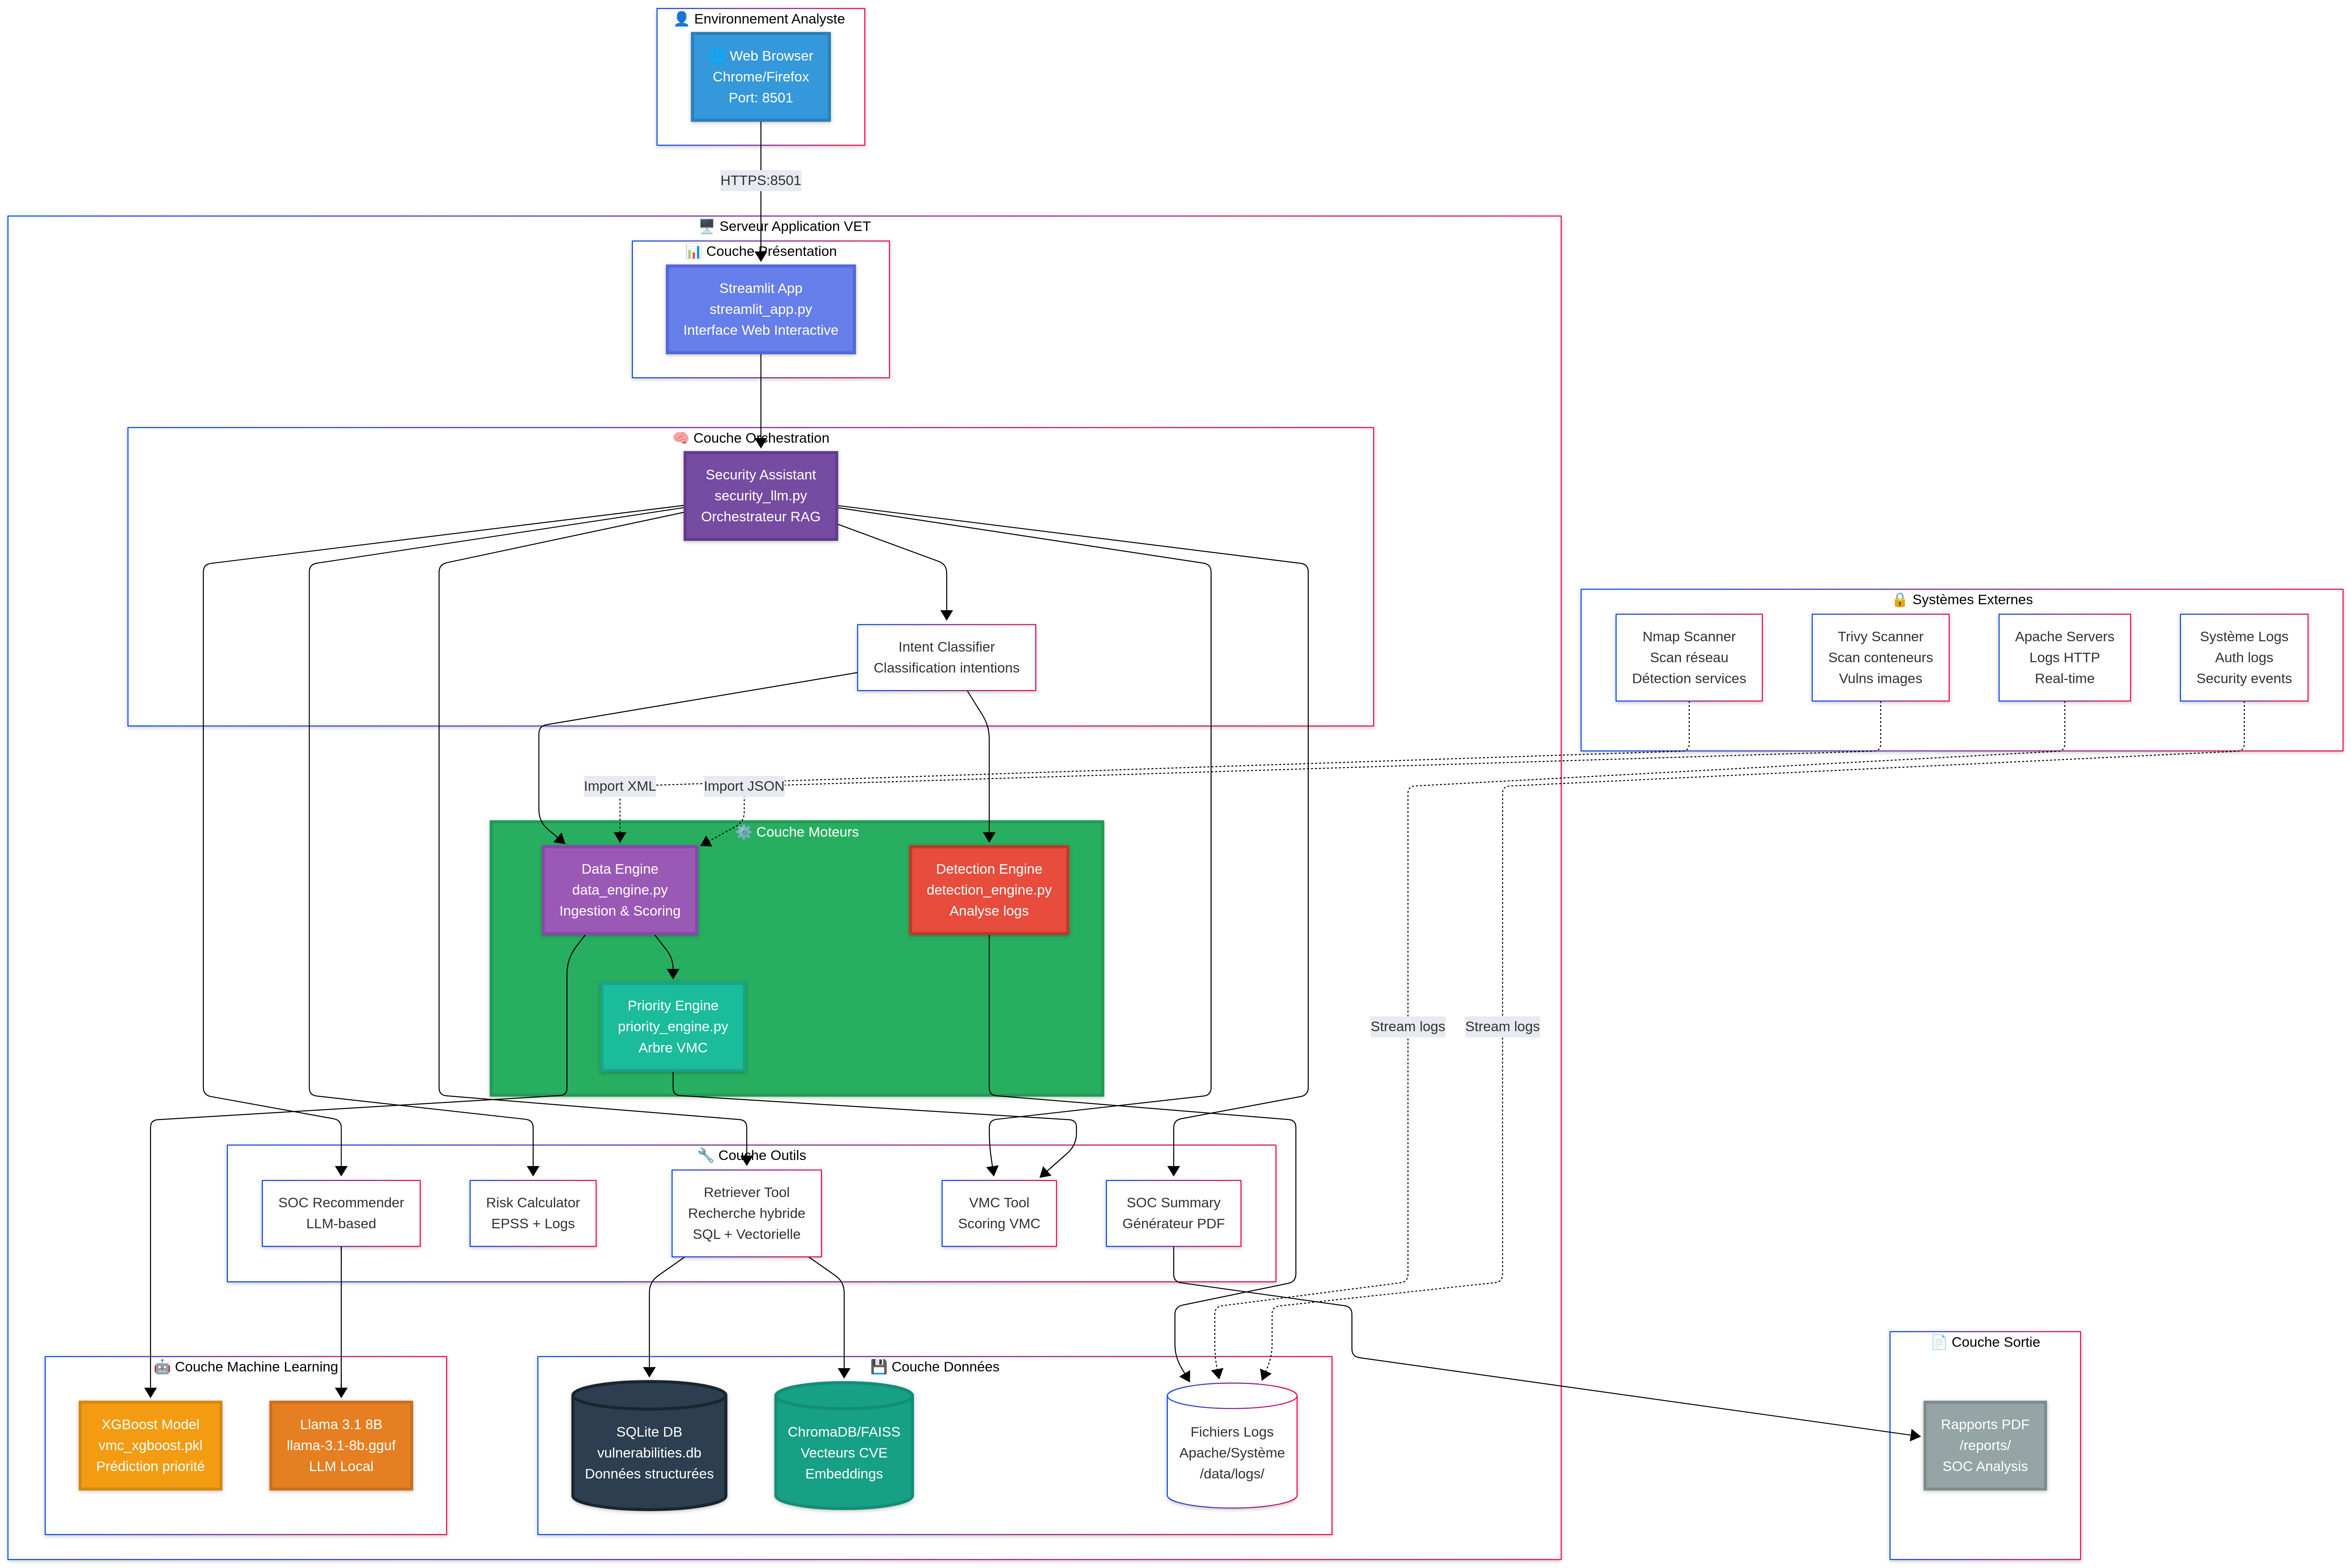
\includegraphics[width=1\textwidth]{img/1.png}
    \caption{Architecture globale du système VET.}
    \label{fig:monimage}
\end{figure}


\subsection{Structure des fichiers}

Le projet est organisé selon la structure suivante~:

\begin{table}[H]
\centering
\footnotesize
\begin{tabular}{l p{8cm}}
\toprule
\textbf{Fichier/Dossier} & \textbf{Rôle} \\
\midrule
\texttt{security\_llm.py} & Agent RAG principal (orchestrateur LangChain) \\
\texttt{data\_engine.py} & Ingestion de données et moteur de scoring VMC/ML \\
\texttt{priority\_engine.py} & Logique de priorisation (arbre de décision VMC) \\
\texttt{detection\_engine.py} & Moteur de détection de traces d'exploitation \\
\texttt{config.py} & Configuration centralisée (LLM, ML, DB, chemins) \\
\texttt{streamlit\_app.py} & Interface Web (Streamlit) \\
\texttt{tools/} & Outils de l'agent (retriever, VMC, risk, recommender, summary) \\
\texttt{utils/} & Modules utilitaires (vectorstore, log\_analyzer) \\
\texttt{data/} & Données (SQLite, ChromaDB, logs, loaders) \\
\texttt{prompts/} & Templates de prompts centralisés \\
\texttt{models/} & Modèles ML (XGBoost) et LLM (GGUF) \\
\bottomrule
\end{tabular}
\caption{Structure des fichiers du projet VET.}
\label{tab:structure}
\end{table}

\subsection{Pipeline de traitement}

Le flux de traitement d'une question utilisateur suit les étapes suivantes~:

\begin{enumerate}[nosep]
    \item \textbf{Réception}~: L'utilisateur pose une question via l'interface Streamlit~\cite{streamlit2023}.
    \item \textbf{Classification d'intention}~: Le LLM classifie la question parmi 8 intentions (\texttt{list\_vulns}, \texttt{analyze\_cve}, \texttt{recommend}, \texttt{logs}, \texttt{search}, \texttt{summary}, \texttt{compromise}, \texttt{general\_security}).
    \item \textbf{Activation des outils}~: Selon l'intention, les outils pertinents sont appelés pour collecter les données nécessaires.
    \item \textbf{Construction du contexte RAG}~: Les résultats des outils sont fusionnés en un contexte structuré dédupliqué.
    \item \textbf{Génération structurée (Pass~1)}~: Le LLM génère une réponse structurée via des schémas Pydantic~\cite{pydantic2023}.
    \item \textbf{Reformulation naturelle (Pass~2)}~: Le LLM reformule la réponse structurée en dialogue naturel pour l'analyste.
\end{enumerate}


% ========================================================================
% 3. INFRASTRUCTURE DE SIMULATION
% ========================================================================
\section{Infrastructure de simulation et d'évaluation}

Pour tester notre solution VET de manière réaliste, nous avons conçu une infrastructure de simulation complète. Celle-ci repose sur un serveur volontairement vulnérable, \textit{FileTransferLike}, qui nous donne la possibilité de générer différents vecteurs d'attaques et de voir si notre IA parvient à les corréler.

\subsection{Architecture et configuration du serveur sous Docker}

L'environnement utilise un conteneur Docker unique (\texttt{getmynote-server}) pour faciliter son déploiement et son orchestration. L'idée est de simuler un serveur d'entreprise accumulant de la dette technique, qui n'aurait pas été mis à jour depuis plusieurs années.

\paragraph{Réalisme et limites.} Il est important de préciser que la nature même de ce conteneur constitue un biais volontaire : il s'agit d'un "pot de miel" de laboratoire particulièrement concentré. Les vulnérabilités qui y sont rassemblées sont extrêmement directes et nombreuses pour un seul système. Cela offre un scénario d'apprentissage idéal pour l'entraînement d'une IA de SOC, bien qu'il soit potentiellement trop dense et asymétrique pour représenter un serveur de production standard. Ce parti pris garantit en revanche un apport massif et immédiat de cas pratiques.

Les choix techniques définis dans notre fichier \texttt{Dockerfile} sont les suivants~:

\begin{itemize}
    \item \textbf{Système d'exploitation}~: \textbf{Ubuntu 18.04}. Son support officiel étant terminé depuis avril 2023, cela nous garantit d'avoir des paquets obsolètes. Nous y avons par exemple forcé l'installation d'une ancienne version de l'interpréteur de commandes Bash pour pouvoir exploiter la fameuse faille Shellshock.
    \item \textbf{Application Web cible}~: Une plateforme de transfert de fichiers développée en \textbf{Python/Flask} autour de 1300 lignes de code et servie par le module \textbf{Apache WSGI} sur le port 8000. 
    \item \textbf{Services réseaux obsolètes}~: Nous avons exposé plusieurs services vulnérables, comme \textbf{MySQL 5.7} avec un compte administrateur sans mot de passe, \textbf{Redis 5.0.3} accessible directement depuis l'extérieur sur l'adresse réseau par défaut, ainsi que \textbf{Samba SMBv1} pour exploiter EternalBlue et \textbf{VSFTPD 3.0.3} qui autorise les envois de fichiers anonymes et inclut une backdoor classique.
    \item \textbf{Mauvaises configurations système}~: Nous avons compilé une ancienne version d'\textbf{OpenSSL} pour simuler Heartbleed. Le système comporte aussi des oublis graves d'administration, comme des droits en lecture et écriture élargis sur le fichier des mots de passe \texttt{/etc/shadow}, l'autorisation de se connecter en SSH en tant qu'administrateur sans mot de passe, ou encore l'usage de la commande \texttt{sudo} sans restriction. Cela facilite considérablement l'exploitation d'une faille locale d'élévation de privilège comme la CVE-2021-3156.
\end{itemize}

\subsection{Choix, répartition et criticité des vulnérabilités}

Au total, l'infrastructure implémente et documente \textbf{89 vulnérabilités}, dont 21 d'infrastructure et 68 applicatives. Ce panel n'est pas aléatoire : il sert à fournir à l'IA une base de référence solide, le ground truth, diversifiée pour couvrir tout le spectre d'une attaque, des failles de criticité faible comme les fuites d'informations aux failles de criticité maximale.

Nous avons réparti ces failles en trois grandes catégories~:
\begin{enumerate}
    \item \textbf{Failles logiques Web}~: On y retrouve les failles majeures du Top 10 OWASP comme les injections SQL, les accès illégitimes aux fichiers via IDOR, et les falsifications de requêtes SSRF. Ce type de failles a été intégré car il génère d'importants volumes de logs HTTP d'erreur sous Apache, fournissant à l'IA des motifs clairs d'injections à analyser dans le trafic entrant.
    \item \textbf{Exécutions de code et Injections SSTI/RCE}~: L'application inclut des injections de templates serveur SSTI, un point de terminaison de diagnostic mal filtré menant à des injections de commandes, ainsi que de la désérialisation Python vulnérable. L'exploitation de ces vecteurs, souvent classée comme critique avec un score CVSS supérieur à 9.0, permet d'aboutir à une exécution de code à distance complète RCE. Cela déclenche des alertes système sous Auditd et l'apparition de processus enfants illégitimes repérables dans la télémétrie.
    \item \textbf{Failles d'infrastructure et post-exploitation}~: L'intégration de protocoles réseau en clair comme Telnet, de bases de données NoSQL non protégées et de failles locales Sudo est primordiale pour valider le modèle. Bien qu'elles soient souvent triviales à exploiter, elles nous permettent de simuler finement les étapes de mouvements latéraux et d'élévation de privilèges, des phases décisives de la kill chain qu'un SOC doit impérativement être capable d'intercepter.
\end{enumerate}

\subsection{Génération de trafic et collecte de télémétrie}

Pour alimenter notre IA en données, nous avons automatisé le cycle de vie des attaques.

Un script d'activité simule le comportement du trafic légitime et malveillant. Il lance des requêtes HTTP ciblées, effectue des scans automatiques avec des outils d'audit comme \textbf{OWASP ZAP}, et réalise des attaques par force brute sur les ports SSH et FTP.

Pour centraliser cette télémétrie, notre conteneur récupère plus de 25 sources de logs différentes grâce aux agents \textbf{Filebeat} et \textbf{Auditbeat}, organisées en trois flux majeurs~:
\begin{itemize}[nosep]
    \item \textbf{Logs Web et Base de données}~: Logs d'accès Apache, traces applicatives de Gunicorn, et un fichier JSON sécuritaire développé en interne où l'application signale elle-même les tentatives d'injections ou comportements anormaux détectés au niveau du code.
    \item \textbf{Logs Système}~: Capture des événements système pour surveiller le téléchargement de charges utiles inattendues, les succès et échecs d'authentification SSH, ainsi que les appels sudo inhabituels.
    \item \textbf{Logs Réseaux}~: Enregistrement des exfiltrations ou des envois de webshells via le service FTP.
\end{itemize}

Un module Python s'occupe ensuite de parser et normaliser ces événements bruts avec la bibliothèque \texttt{pyGrok}. Tout est formaté en JSON, ce qui prépare le format d'ingestion adéquat pour notre modèle de détection de Machine Learning.

\subsection{Évaluation par scanners, validation et analyse comparative}

Afin d'obtenir une base de comparaison solide pour le projet, nous avons audité notre environnement de test avec trois scanners industriels de référence. Cette analyse croisée permet à la fois de garantir que notre architecture répond bien aux attaques automatisées classiques, et de confronter notre déploiement initial de vulnérabilités à ce qui ressort de scans professionnels effectifs.

\begin{table}[H]
\centering
\small
\begin{tabular}{l l p{6.5cm}}
\toprule
\textbf{Outil} & \textbf{Approche de scan} & \textbf{Visibilité sur l'infrastructure} \\
\midrule
\textbf{OWASP ZAP} & Scan Web Actif DAST & Cible l'application Flask et confirme de manière catégorique la présence des vulnérabilités web intégrées SQLi, CSRF, SSTI. \\
\textbf{OpenVAS} & Audit d'Infrastructure & Évalue la surface réseau, la robustesse des services exposés et identifie les faillibilités matérielles. \\
\textbf{Trivy} & Scan de conteneurs SCA & Liste les dépendances système et logicielles obsolètes liées à l'image Ubuntu 18.04 et examine le code source. \\
\bottomrule
\end{tabular}
\caption{Outils d'audit utilisés et périmètre couvert sur FileTransferLike.}
\label{tab:scantools}
\end{table}

\paragraph{Analyse des détections et concordances.} La compilation de ces rapports génère plus de 175 alertes distinctes sur l'ensemble du périmètre. L'étude détaillée des occurrences démontre la fiabilité du protocole de simulation :

\begin{itemize}
    \item \textbf{Succès de la Détection DAST avec OWASP ZAP} : ZAP remonte avec pertinence des failles logiques très attendues. L'analyse de son rapport identifie avec succès l'Injection SQL sur la page de connexion, le Server Side Template Injection intégré dans le moteur de rendus HTML, et détecte correctement l'absence de jetons Anti-CSRF voulue lors des suppressions de comptes, ainsi que de multiples redirections ouvertes. L'exposition flagrante des commentaires noyés dans notre code et l'absence radicale d'en-têtes de sécurité sont également explicitement signalées.
    
    \item \textbf{Exploration Réseau par OpenVAS} : Ce scanner assure son rôle en identifiant plusieurs vulnérabilités fondamentales créées exprès sur le conteneur, telles que la présence du protocole Telnet transmettant des informations en clair ou les lacunes sur le port FTP et la surface de débogage du réseau cible.
    
    \item \textbf{Analyse Structurelle via Trivy} : Enfin, le scan de composition corrobore parfaitement notre implémentation de logiciels délibérément affaiblis. Le rapport recense exhaustivement l'historique des CVE lié à notre distribution Bionic Beaver obsolète et note formellement toute l'étendue des bibliothèques Python à risque.
\end{itemize}

Cet alignement entre les vulnérabilités sciemment documentées dans notre matrice de référence et leurs identifications directes par les scanners confirme l'excellence de FileTransferLike en tant que jeu de données qualifié. Les failles ne sont pas seulement théoriques, elles sont tangibles, mesurables par des tiers, et garantissent la solidité du corpus pour l'entraînement de VET.


% ========================================================================
% 4. INGESTION DES DONNÉES
% ========================================================================
\section{Ingestion des données}

\subsection{Base de données SQLite}

Le module \texttt{cve\_loader.py} gère la création et l'alimentation de la base de données SQLite~\cite{sqlite2024} qui contient deux tables principales~:

\paragraph{Table \texttt{cve} (table centrale).} Elle stocke toutes les informations techniques d'une vulnérabilité~: identifiant CVE, description, scores CVSS et EPSS, vecteur d'attaque, CWE, vendeur, produit, et statut KEV.

\paragraph{Table \texttt{server\_vulns} (liaison serveur-CVE).} Elle trace quelles CVE affectent quels serveurs dans l'infrastructure, permettant une analyse contextuelle.

\subsection{Sources de données}

L'enrichissement de la base de données s'effectue en quatre phases~:

\begin{enumerate}[nosep]
    \item \textbf{Collecte NVD}~\cite{nvd2024}~: Téléchargement via l'API NVD~2.0, filtré par mots-clés liés aux serveurs HTTP/Web (Apache, Nginx, Flask, Tomcat, etc.). Chaque CVE est parsée pour extraire le CVSS ($\geq$ v3.1), le CWE, et les CPE (vendeur/produit).
    \item \textbf{Enrichissement KEV}~\cite{cisa_kev2024}~: Le catalogue CISA KEV est téléchargé et croisé avec la base. Chaque CVE connue comme activement exploitée est marquée avec \texttt{in\_kev=1}.
    \item \textbf{Scores EPSS}~\cite{epss2023}~: Les scores EPSS (Exploit Prediction Scoring System) sont téléchargés par lots de 30 CVE via l'API FIRST.org, fournissant une probabilité d'exploitation à 30 jours.
    \item \textbf{Mapping Trivy}~: Le rapport XML généré par Trivy~\cite{trivy2024} est parsé par \texttt{trivy\_loader.py} pour peupler la table \texttt{server\_vulns}.
\end{enumerate}

\subsection{Indexation vectorielle (RAG)}

Pour permettre la recherche sémantique, les descriptions des CVE sont transformées en vecteurs d'embedding et indexées~:

\paragraph{Modèle d'embedding.} Le modèle \texttt{all-MiniLM-L6-v2}~\cite{reimers2019sentencebert} (Sentence Transformers) transforme chaque description de CVE en un vecteur dense de 384 dimensions.

\paragraph{Vectorstore FAISS.} FAISS (Facebook AI Similarity Search)~\cite{johnson2019faiss} est utilisé comme base de données vectorielle pour sa rapidité de recherche approchée (ANN). L'index est construit par le module \texttt{utils/vectorstore.py}, qui~:
\begin{enumerate}[nosep]
    \item Récupère toutes les descriptions CVE depuis SQLite,
    \item Crée des documents LangChain avec métadonnées (CVSS, EPSS, KEV, vendeur),
    \item Indexe via \texttt{FAISS.from\_documents()},
    \item Sauvegarde l'index localement pour chargement rapide ultérieur.
\end{enumerate}


% ============================================================
% Section 5 — Moteur de priorisation : VMC et XGBoost
% Style LNCS — à insérer dans le rapport principal
% ============================================================

\section{Moteur de priorisation : VMC et XGBoost}

\subsection{Pourquoi on a besoin d'un moteur de priorisation ?}

Quand on travaille dans un SOC, le vrai problème ce n'est pas de trouver les vulnérabilités. Les scanners font ça très bien. Le vrai problème, c'est de savoir lesquelles traiter en premier.

Sur notre serveur vulnérable, on a trouvé 175 vulnérabilités avec les outils de scan (OWASP ZAP, OpenVAS, Trivy). On en a gardé 25 pour les tests. Mais même avec 25 vulnérabilités, si on les trie uniquement par score CVSS, on se retrouve avec beaucoup de \og CRITIQUE \fg{} alors que certaines ne seront jamais exploitées dans la réalité.

C'est pour ça qu'on a mis en place un moteur de priorisation qui combine plusieurs sources d'information pour donner un score plus réaliste.

% ------------------------------------------------------------
\subsection{Le framework VMC (Vulnerability Management Chaining)}

\subsubsection{Principe général.}

VMC est un arbre de décision. L'idée vient d'un article scientifique de Shimizu et Hashimoto~\cite{shimizu2023vmc} qui montre que combiner CVSS, EPSS et KEV permet de réduire jusqu'à 95\% le nombre de vulnérabilités \og urgentes \fg{} à traiter, tout en gardant une bonne couverture des vraies menaces.

Le principe repose sur quatre questions, posées dans l'ordre suivant :
\begin{enumerate}
    \item La vulnérabilité est-elle dans le catalogue KEV de la CISA ? Si oui, c'est une menace confirmée avec exploitation active.
    \item Sinon, son score EPSS est-il élevé ? Plus le score est haut, plus il y a de chances qu'elle soit exploitée dans les 30 prochains jours.
    \item Quel est son impact technique selon le CVSS ?
    \item La vulnérabilité permet-elle une exécution de code à distance (RCE) ? Le serveur est-il critique ?
\end{enumerate}

\subsubsection{Le calcul du score VMC.}

Dans notre implémentation (fichier \texttt{priority\_engine.py}), on calcule un score entre 0 et 100 selon la formule suivante :

\begin{equation}
    S_{VMC} = (CVSS \times 4) + (20 \cdot \mathbb{1}_{KEV}) + (EPSS \times 20) + (10 \cdot \mathbb{1}_{RCE}) + 5
    \label{eq:vmc}
\end{equation}

Ce score se décompose en trois composantes pondérées :
\begin{itemize}
    \item \textbf{Base (40\%)} : le score CVSS multiplié par 4. Comme CVSS varie de 0 à 10, cette composante contribue jusqu'à 40 points et mesure la gravité technique de la faille.
    \item \textbf{Menace (40\%)} : 20 points si la CVE figure dans le catalogue KEV (exploitation confirmée dans la nature), plus jusqu'à 20 points selon le score EPSS. Par exemple, un EPSS de 0.5 ajoute 10 points.
    \item \textbf{Contexte (20\%)} : 10 points si la description contient des indicateurs de RCE, et 5 points fixes pour la criticité du serveur.
\end{itemize}

\subsubsection{Classification en niveaux de priorité.}

Une fois le score calculé, chaque vulnérabilité est classifiée dans l'un des quatre niveaux décrits dans le Tableau~\ref{tab:vmc_levels}.

\begin{table}[h]
\centering
\caption{Niveaux de priorité VMC}
\label{tab:vmc_levels}
\begin{tabular}{|c|c|l|}
\hline
\textbf{Score VMC} & \textbf{Niveau} & \textbf{Interprétation} \\
\hline
$\geq 90$ & CRITIQUE & Action immédiate requise \\
$\geq 70$ & HAUTE    & Traitement prioritaire \\
$\geq 40$ & MOYENNE  & À planifier \\
$< 40$    & FAIBLE   & Surveillance simple \\
\hline
\end{tabular}
\end{table}

Pour illustrer l'apport de cette approche par rapport au CVSS seul : une CVE avec CVSS 9.8, présente dans KEV, EPSS à 0.85, et permettant un RCE obtient un score VMC proche de 100 — clairement CRITIQUE. En revanche, une CVE avec CVSS 9.0 mais EPSS à 0.001 et absente du catalogue KEV obtient un score autour de 36 — théoriquement grave, mais concrètement peu risqué.

% ------------------------------------------------------------
\subsection{La couche Machine Learning : XGBoost}

\subsubsection{Pourquoi ajouter du Machine Learning ?}

L'arbre de décision VMC fournit une baseline claire et explicable, mais il a une limite : ses règles sont fixes. Il ne capture pas les interactions complexes entre les variables. Par exemple, il ne détecte pas facilement qu'un vendeur particulier combiné à un type de faille spécifique présente historiquement un profil d'exploitation plus dangereux.

C'est pour cette raison qu'on a ajouté une couche XGBoost dans \texttt{data\_engine.py}. XGBoost est un algorithme de gradient boosting : au lieu de construire un seul arbre de décision, il en construit des centaines en séquence, chaque arbre corrigeant les erreurs du précédent. Ce mécanisme lui permet d'apprendre des patterns non linéaires que des règles fixes ne peuvent pas capturer.

\subsubsection{Génération des données d'entraînement.}

Un défi classique en apprentissage supervisé est la disponibilité de données labellisées. Dans notre contexte, on ne disposait pas d'exemples annotés par des analystes. La solution adoptée est une \textbf{supervision automatique} : on utilise les décisions de l'arbre VMC comme labels d'entraînement. Pour chaque CVE dans la base de données, on applique les règles VMC pour obtenir une priorité (CRITICAL, HIGH, MEDIUM, LOW), et c'est cette priorité qui devient le label fourni à XGBoost.

Cette approche permet à XGBoost de généraliser les règles métier VMC, en capturant des interactions que l'arbre simple ne détecterait pas — par exemple, qu'une vulnérabilité Apache avec une injection SQL est souvent dangereuse même si l'EPSS n'est pas très élevé.

\subsubsection{Features utilisées.}

Le modèle XGBoost s'appuie sur cinq features décrites dans le Tableau~\ref{tab:features}.

\begin{table}[h]
\centering
\caption{Features utilisées par le modèle XGBoost}
\label{tab:features}
\begin{tabular}{|l|c|l|}
\hline
\textbf{Feature} & \textbf{Type} & \textbf{Description} \\
\hline
\texttt{cvss\_score}    & Numérique (0--10) & Score de sévérité technique \\
\texttt{epss\_score}    & Numérique (0--1)  & Probabilité d'exploitation à 30 jours \\
\texttt{in\_kev}        & Binaire (0/1)     & Présence dans le catalogue KEV \\
\texttt{vendor\_encoded} & Catégoriel encodé & Vendeur (Apache=1, Nginx=2, Microsoft=3\ldots) \\
\texttt{cwe\_encoded}   & Catégoriel encodé & Type de faille (SQLi=1, XSS=2, RCE=3\ldots) \\
\hline
\end{tabular}
\end{table}

Ces features combinent des informations quantitatives (les scores) avec des informations qualitatives (vendeur, type de faille). Ce choix s'inspire des résultats du modèle EPSS v3~\cite{jacobs2023epss}, qui montre que les signaux les plus prédictifs de l'exploitation incluent justement les mots-clés dans la description, le vendeur, et la présence dans des listes d'exploitation connues.

\subsubsection{Processus d'entraînement.}

L'entraînement est implémenté dans la méthode \texttt{train\_xgboost()} de la classe \texttt{VMCXGBoostEngine} et se déroule en six étapes :

\begin{enumerate}
    \item Chargement de toutes les CVE depuis la base de données SQLite via le \texttt{PriorityEngine}.
    \item Application des règles VMC pour générer les labels de classification.
    \item Encodage des variables catégorielles avec un \texttt{LabelEncoder}.
    \item Division des données : 80\% pour l'entraînement, 20\% pour le test.
    \item Entraînement XGBoost en classification multi-classes (\texttt{objective='multi:softprob'}, \texttt{max\_depth=6}, \texttt{learning\_rate=0.1}, \texttt{n\_estimators=100}).
    \item Sauvegarde du modèle et des encodeurs avec \texttt{joblib}.
\end{enumerate}

\subsubsection{Prédiction et mécanisme de fallback.}

Lors de l'inférence, le modèle calcule une probabilité pour chacune des quatre classes et retourne la classe avec la probabilité la plus élevée, accompagnée d'un score de confiance. Un mécanisme de fallback est intégré : \textbf{si la confiance est inférieure à 80\%}, le système affiche également l'avis de l'arbre VMC. L'analyste peut ainsi voir les deux opinions et trancher.

Ce design respecte le principe du \textit{Human In The Loop}~\cite{cyberally2024} : le modèle propose, mais le jugement humain reste central.

% ------------------------------------------------------------
\subsection{L'orchestration : le VMC Tool}

Le fichier \texttt{vmc\_tool.py} joue le rôle de coordonnateur. C'est lui qui est appelé par l'agent LangChain lorsque l'analyste pose une question sur les vulnérabilités. Son fonctionnement suit quatre étapes :

\begin{enumerate}
    \item Appel au \texttt{PriorityEngine} pour récupérer la liste des CVE avec leurs scores VMC.
    \item Pour chaque CVE, demande d'une prédiction XGBoost à la couche ML.
    \item Construction d'un contexte enrichi pour le LLM, avec variables structurées (nombre de critiques, CVE la plus dangereuse, EPSS moyen).
    \item Formatage en texte clair pour Llama 3.1. Exemple :
\end{enumerate}

\begin{verbatim}
1. CVE-2021-44228 [CRITIQUE] (VMC: 95.0)
   EPSS: 0.9750, KEV: OUI
   Apache Log4j remote code execution...
\end{verbatim}

Ce format compact permet au LLM de comprendre rapidement la situation et de formuler une réponse justifiée pour l'analyste.

% ------------------------------------------------------------
\subsection{Avantages de l'approche hybride}

La combinaison VMC et XGBoost apporte plusieurs avantages concrets :

\begin{itemize}
    \item \textbf{Transparence} : l'arbre VMC est toujours explicable. On peut justifier chaque décision par ses composantes (KEV, EPSS, CVSS), ce qui est essentiel pour la confiance de l'analyste.
    \item \textbf{Flexibilité} : XGBoost capture des patterns que les règles fixes ne voient pas, comme des combinaisons de vendeur et type de faille historiquement plus exploitées.
    \item \textbf{Fiabilité} : le mécanisme de fallback garantit qu'on a toujours une réponse exploitable. En cas de faible confiance, l'analyste dispose des deux avis.
    \item \textbf{Cohérence} : comme XGBoost est entraîné sur les décisions VMC, les deux systèmes ne se contredisent pas fondamentalement. XGBoost raffine les règles VMC sans les remplacer.
\end{itemize}

% ------------------------------------------------------------
\subsection{Résultats observés sur notre dataset}

Sur les 25 vulnérabilités de test issues de notre serveur Docker, le moteur a produit une distribution cohérente avec les attentes. Les CVE ayant obtenu les scores les plus élevés sont :

\begin{itemize}
    \item \textbf{CVE-2004-2687} (DistCC RCE) : présente dans KEV, EPSS élevé, RCE confirmé $\rightarrow$ score VMC $\approx$ 95.
    \item \textbf{CVE-2017-0144} (EternalBlue/SMBv1) : présente dans KEV, associée à des campagnes de ransomware actives $\rightarrow$ niveau CRITIQUE.
    \item \textbf{CVE-2014-6271} (Shellshock) : présente dans KEV, code d'exploitation très répandu $\rightarrow$ niveau CRITIQUE.
\end{itemize}

À l'opposé, des vulnérabilités avec un CVSS élevé mais sans exploitation confirmée (absentes de KEV, EPSS faible) ont été classées MOYENNE ou FAIBLE. Ce résultat est cohérent avec les conclusions de~\cite{shimizu2023vmc} : l'approche permet de réduire de 95\% le volume de vulnérabilités \og urgentes \fg{} tout en maintenant une couverture de 85\% des vraies menaces, aidant ainsi l'analyste à concentrer son attention sur les risques réels.


% ========================================================================
% 6. SYSTÈME RAG ET AGENT LLM
% ========================================================================
\section{Système RAG et Agent LLM}

\subsection{Architecture RAG}

Le système RAG (Retrieval-Augmented Generation)~\cite{lewis2020rag} constitue le c\oe{}ur intelligent de VET. Il permet au LLM de répondre avec précision en s'appuyant sur des données factuelles extraites de la base de connaissances, plutôt que de s'appuyer uniquement sur ses connaissances pré-entraînées.

\paragraph{Modèle LLM.} VET utilise le modèle \textbf{Llama~3.1~8B}~\cite{llama3_2024} de Meta, exécuté localement via \texttt{llama.cpp}~\cite{llamacpp2024} au format quantifié GGUF (Q5\_K\_M). Ce choix garantit~:
\begin{itemize}[nosep]
    \item \textbf{Confidentialité}~: aucune donnée ne quitte l'infrastructure (pas d'API cloud),
    \item \textbf{Performance}~: temps de réponse acceptable avec accélération GPU,
    \item \textbf{Qualité}~: le modèle 8B offre un bon équilibre entre taille et capacité d'analyse complexe.
\end{itemize}

La configuration du LLM est centralisée dans \texttt{config.py}~: température basse (0.1) pour la reproductibilité, contexte de 8192 tokens, et pénalité de répétition de 1.2.

\subsection{Outils de l'agent}

L'agent \texttt{SecurityAssistant} orchestre cinq outils spécialisés, chacun implémentant l'interface \texttt{StructuredTool} de LangChain~\cite{langchain2023}~:

\begin{table}[H]
\centering
\footnotesize
\begin{tabular}{l p{3cm} p{5.5cm}}
\toprule
\textbf{Outil} & \textbf{Module} & \textbf{Fonction} \\
\midrule
CVE RAG Search & \texttt{retriever\_tool.py} & Recherche hybride SQL + vectorielle \\
VMC Priorities & \texttt{vmc\_tool.py} & Classement VMC + scores XGBoost \\
Risk Calculator & \texttt{risk\_calculator.py} & Score de risque dynamique (EPSS + logs) \\
SOC Recommender & \texttt{soc\_recommender.py} & Recommandations contextuelles SOC \\
SOC Summary & \texttt{soc\_summary.py} & Génération de rapports PDF automatiques \\
\bottomrule
\end{tabular}
\caption{Outils de l'agent SecurityAssistant.}
\label{tab:tools}
\end{table}

\subsection{Recherche hybride}

Le \texttt{ServerHybridRetriever} implémente une stratégie de recherche en trois étapes~:

\begin{enumerate}[nosep]
    \item \textbf{Requête SQL}~: Récupération des CVE associées au serveur cible depuis \texttt{server\_vulns},
    \item \textbf{Filtrage vectoriel}~: Si des CVE serveur sont trouvées, recherche sémantique FAISS filtrée sur ces CVE (top~100 résultats, filtrage Python, rétention des top~8),
    \item \textbf{Fallback global}~: Si aucun résultat n'est trouvé pour le serveur, recherche vectorielle globale (top~8).
\end{enumerate}

Cette approche garantit la pertinence contextuelle~: les résultats sont toujours liés au serveur analysé, tout en permettant un fallback vers la base complète si nécessaire.

\subsection{Classification d'intention}

Le système utilise un mécanisme de classification d'intention en deux couches~:

\paragraph{Override par règles.} Avant tout appel au LLM, des règles déterministes détectent certaines intentions via des expressions régulières~:
\begin{itemize}[nosep]
    \item Détection de pattern CVE (\texttt{CVE-\textbackslash d\{4\}-\textbackslash d+}) $\rightarrow$ intention \texttt{analyze\_cve},
    \item Mots-clés de logs (\texttt{logs}, \texttt{traces}, \texttt{exploitation}) $\rightarrow$ intention \texttt{logs}.
\end{itemize}

\paragraph{Classification LLM.} Pour les cas non couverts par les règles, le LLM classifie l'intention en retournant un JSON structuré~: \texttt{\{security, intent, confidence\}}.

\subsection{Génération structurée (2-Pass LLM)}

VET utilise une architecture à deux passes~:

\paragraph{Pass~1 --- Analyse structurée.} Le LLM génère une réponse conforme à un schéma Pydantic~\cite{pydantic2023}. Par exemple, pour l'intention \texttt{list\_vulns}, le schéma \texttt{CVEClassement} impose~:
\begin{itemize}[nosep]
    \item \texttt{total\_vulns}~: nombre total de vulnérabilités,
    \item \texttt{top\_recommendation}~: CVE la plus dangereuse,
    \item \texttt{prioritized\_list}~: liste structurée des top~3 CVE avec EPSS, KEV, description.
\end{itemize}

\paragraph{Pass~2 --- Reformulation naturelle.} La sortie structurée est ensuite reformulée par le LLM en dialogue naturel, adapté au rôle de l'interlocuteur (analyste SOC).

\subsection{Calcul de risque dynamique}

Le \texttt{risk\_calculator.py} implémente un calcul de risque combinant EPSS et analyse de logs~:

\begin{equation}
P(\text{exploit}) = P(\text{EPSS}) + P(\text{logs}) - P(\text{EPSS}) \times P(\text{logs})
\label{eq:risk}
\end{equation}

Cette formule correspond à la probabilité de l'union de deux événements ($P(A \cup B)$). Le facteur log est fixé à 0.9 en cas d'exploitation détectée et 0.4 en cas d'activité suspecte.

\subsection{Analyse de logs}

Le module \texttt{SecurityLogAnalyzer} dans \texttt{utils/log\_analyzer.py} analyse les logs de sécurité en temps réel pour détecter des patterns d'attaque~:

\begin{itemize}[nosep]
    \item \textbf{Injection SQL}~: Détection de patterns comme \texttt{UNION SELECT}, \texttt{1=1}, \texttt{OR 1=1},
    \item \textbf{XSS}~: Recherche de balises \texttt{<script>} et encodages malveillants,
    \item \textbf{Traversée de répertoire}~: Détection de \texttt{../} et variantes encodées,
    \item \textbf{Injection de commandes}~: Patterns de pipe (\texttt{|}), point-virgule, backticks,
    \item \textbf{Force brute}~: Comptage de tentatives échouées par IP source.
\end{itemize}

L'analyse produit un rapport structuré incluant~: le statut d'exploitation, le nombre de tentatives suspectes, les IP sources, et les types d'attaque détectés.

\subsection{Interface utilisateur Streamlit}

L'interface est développée avec Streamlit~\cite{streamlit2023} et offre~:
\begin{itemize}[nosep]
    \item Un \textbf{chat conversationnel} avec mémoire (historique de conversation),
    \item Un \textbf{tableau de bord} de distribution des risques (VMC),
    \item La \textbf{génération de rapports PDF} téléchargeables,
    \item Un sélecteur de serveur pour l'analyse contextuelle.
\end{itemize}


% ========================================================================
% 7. TRAVAUX CONNEXES
% ========================================================================
\section{Travaux connexes}

\subsection{Systèmes de gestion des vulnérabilités}

Les outils commerciaux de gestion des vulnérabilités (Qualys, Tenable Nessus, Rapid7 InsightVM) fournissent des capacités de scan et de priorisation. Cependant, leur approche de priorisation repose principalement sur le score CVSS, sans intégrer de manière native~:
\begin{itemize}[nosep]
    \item La corrélation avec les logs d'exploitation réels,
    \item L'analyse conversationnelle en langage naturel,
    \item Le Machine Learning pour la priorisation adaptative.
\end{itemize}

VET se différencie en combinant ces trois aspects dans un assistant conversationnel unifié.

\subsection{RAG pour la cybersécurité}

Le paradigme RAG~\cite{lewis2020rag}, initialement proposé pour les tâches NLP knowledge-intensive, a été appliqué dans plusieurs contextes de cybersécurité, notamment pour l'analyse de rapports de menaces (threat intelligence) et la classification de malwares. VET adapte ce paradigme au contexte SOC en utilisant une base de connaissances structurée (CVE + EPSS + KEV) plutôt que des documents texte bruts.

\subsection{ML pour la priorisation de vulnérabilités}

L'utilisation du Machine Learning pour la priorisation des vulnérabilités est un domaine de recherche actif. Les travaux récents explorent les modèles de gradient boosting (XGBoost, LightGBM) pour prédire l'exploitabilité des CVE à partir de features textuelles et structurées. VET adopte XGBoost~\cite{chen2016xgboost} avec une approche originale~: l'entraînement supervisé automatique à partir des décisions de l'arbre VMC, créant ainsi un système où le ML apprend et généralise les règles métier.

\subsection{Comparaison des approches}

\begin{table}[H]
\centering
\footnotesize
\begin{tabular}{l c c c c}
\toprule
\textbf{Critère} & \textbf{VET} & \textbf{Qualys} & \textbf{Nessus} & \textbf{InsightVM} \\
\midrule
Priorisation CVSS & \checkmark & \checkmark & \checkmark & \checkmark \\
Intégration EPSS & \checkmark & Partiel & Non & Partiel \\
Catalogue KEV & \checkmark & \checkmark & Non & \checkmark \\
Corrélation logs & \checkmark & Non & Non & Partiel \\
ML (XGBoost) & \checkmark & Non & Non & Non \\
Interface NLP & \checkmark & Non & Non & Non \\
LLM local & \checkmark & Non & Non & Non \\
Open-source & \checkmark & Non & Non & Non \\
\bottomrule
\end{tabular}
\caption{Comparaison de VET avec les solutions commerciales.}
\label{tab:comparison}
\end{table}

Les principaux avantages de VET sont l'intégration d'un LLM local pour le dialogue en langage naturel et la combinaison de priorisation ML avec corrélation de logs. Les limitations incluent le périmètre de scan (dépendant d'outils tiers) et la nécessité de ressources GPU pour des performances optimales.


% ========================================================================
% 8. CONCLUSION ET PERSPECTIVES
% ========================================================================
\section{Conclusion et perspectives}

\subsection{Bilan}

Le projet VET démontre la faisabilité d'un assistant SOC intelligent, capable d'analyser et de prioriser les alertes de sécurité en combinant un grand modèle de langage localisé, une architecture RAG et un moteur de priorisation hybride. Les principaux résultats de cette implémentation sont~:

\begin{itemize}
    \item \textbf{Un pipeline RAG contextuel de bout en bout}~: Le système couvre tout le processus, de l'ingestion des bases de vulnérabilités NVD jusqu'au dialogue de réponse. L'utilisation d'une recherche hybride, alliant ciblage SQL précis puis filtrage vectoriel via FAISS, permet d'assurer que l'IA répond toujours en se basant sur la réalité technique du serveur ciblé.
    \item \textbf{Un moteur de priorisation hybride explicable}~: Nous avons combiné une approche déterministe sous forme d'arbre de décision, le Vulnerability Metric Classifier exploitant le CVSS, l'EPSS et le KEV, à un modèle XGBoost. XGBoost apprend des décisions de l'arbre pour les généraliser, ce qui nous a permis de filtrer drastiquement les urgences sans compromettre la détection des menaces avérées.
    \item \textbf{Une corrélation Logs et Vulnérabilités dynamique}~: L'innovation clé réside dans la pondération des faits réels. Une vulnérabilité critique théorique devient une alerte absolue et son score bondit si notre analyseur détecte des traces d'attaques correspondantes dans les logs, par exemple des motifs d'injection SQL sur une application vulnérable.
    \item \textbf{Une génération structurée en architecture double passe}~: VET contraint d'abord le LLM avec des schémas Pydantic pour s'assurer que les données extraites sont fiables et au bon format, comme les listes de CVE et les indicateurs de risque. Ensuite, une deuxième passe LLM reformule ces résultats bruts en un langage naturel et professionnel.
    \item \textbf{Un outil respectueux de la confidentialité}~: En exploitant le modèle Llama 3.1 8B exécuté localement, on garantit qu'aucune donnée de production sensible de l'entreprise, tels que les journaux, adresses IP ou infrastructures, n'est envoyée vers des serveurs tiers ou des API cloud grand public.
\end{itemize}

\subsection{Défis et obstacles rencontrés}

La conception de VET s'est heurtée à plusieurs complexités techniques liées à la nature même de l'IA générative~:

\begin{itemize}
    \item \textbf{Les hallucinations du LLM et le formatage}~: Avec un modèle de la taille de Llama 8B, nous avions des dérives où le LLM inventait des données sur les CVE ou cassait les structures JSON attendues. L'implémentation de la méthode à double passe et de consignes strictes dans les prompts, comme l'interdiction formelle d'inventer des données, a considérablement fiabilisé le système.
    \item \textbf{La classification des intentions de l'utilisateur}~: L'outil devant choisir la bonne procédure entre lire les logs, interroger le NVD ou faire un résumé, laisser le LLM deviner l'intention cible générait des erreurs de routage. Nous l'avons pallié par un filtrage basique mais robuste en amont : des expressions régulières qui forcent le choix de l'outil approprié si la demande est évidente avec des mots-clefs précis liés aux CVE.
    \item \textbf{La fluidité du dialogue face à un format structuré}~: Réussir à garder un dialogue naturel avec l'utilisateur tout en imposant au système un format d'extraction de données très rigide a été un vrai défi de développement. C'est précisément pour cela que l'architecture technique à double passe est devenue incontournable, elle sépare l'extraction pure de la formulation conversationnelle.
\end{itemize}

\subsection{Perspectives d'évolution}

Plusieurs améliorations pourraient être envisagées pour rapprocher ce prototype des standards de la production~:

\begin{itemize}
    \item \textbf{Le Human-in-the-Loop et l'amélioration continue}~: L'idée est de permettre à un analyste senior SOC de faire des retours explicites sur les réponses de l'IA. Si le modèle propose une recommandation, l'analyste devrait pouvoir la corriger ou lui indiquer de nouveaux éléments. L'IA pourrait ainsi réviser son analyse en direct et intégrer cet avis critique pour affiner son contexte de réponse lors des sollicitations futures.
    \item \textbf{Orchestration améliorée et corrélation croisée via LangGraph}~: Le passage à un orchestrateur plus puissant permettrait au système d'utiliser une chaîne d'informations plus intelligemment. L'IA pourrait croiser par elle-même les différents outils pour assurer une bien meilleure mise en contexte, par exemple en cherchant une CVE de manière isolée pour ensuite aller chercher les adresses IP correspondantes dans les logs, garantissant ainsi une corrélation redoutablement plus riche lors d'incidents complexes.
    \item \textbf{Adoption de modèles spécialisés}~: Le modèle de test Llama 3.1 8B est généraliste. Le remplacer par un modèle de plus grande dimension ou, idéalement, un modèle ayant subi un apprentissage spécifique sur la rhétorique et les documents propres à la cybersécurité ferait bondir la qualité rédactionnelle et d'analyse.
    \item \textbf{Intégration SIEM en temps réel}~: Notre analyseur de logs fonctionnant actuellement avec des exports statiques textuels, la suite logique serait de connecter directement VET à des solutions du marché comme Elastic ou Splunk pour le traitement automatique du flux en temps réel.
\end{itemize}


% ========================================================================
% BIBLIOGRAPHIE
% ========================================================================
\newpage
\bibliography{biblioFile}
\bibliographystyle{splncs04}

\end{document}
